\documentclass{article}

\usepackage{array}
\usepackage{graphicx}

\begin{document}

\title{Magnetic Moments}
\author{GSI: Caleb Eades}
\date{11/8}
\maketitle

\section{Midterm Example Problems}

\subsection{Spinning Rods}

A uniformly charged rod of length $L$ and charge $Q$ spins at angular velocity $\omega$ about an axis through the center of the rod perpendicular to the length.
\begin{itemize}
	\item[(a)] Calculate the magnetic moment.
	\item[(b)] If a uniform magnetic field $\vec{B}=B_0\hat{z}$ is present, what is the torque on and potential energy of this rod.
\end{itemize}

\textit{Source: modified from Packard Final Exam, Spring 2000, question 4}

\subsection{Non-uniform Field}

A rigged square current loop with sides $s$, current $I$, and mass $m$ is on a table with coefficient of static friction $\mu_s$. The magnetic field is pointed along the vertical direction, and has magnitude that increases linearly with position: $\vec{B}=B_0\frac{x}{a}\hat{y}$, for a constant $a$. What is the minimum that $\mu_s$ can be if the loop does not move?

\textit{Source: Speliotopoulos Final Exam, Fall 2012, question 4}

\subsection{Levitating Rings?}

A ring of radius $R$, charge $Q$ and mass $M$ is spinning around its symmetry axis. The ring sits on a horizontal frictionless surface. A uniform external magnetic field of strength $B$ is parallel to the plane of the ring. Find the angular velocity $\omega$ at which there is zero normal force between one edge of the ring and the surface.

\begin{figure}[h]
	\begin{center}
		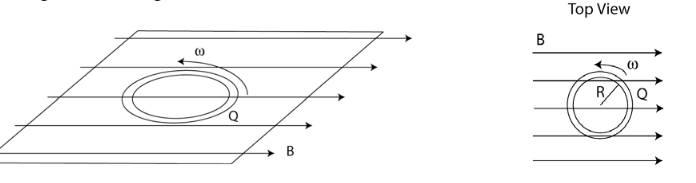
\includegraphics[width=0.9\textwidth]{Ring.png}
	\end{center}
\end{figure}

\textit{Source: Packard Final Exam, Fall 2004, question 1}

\end{document}
